\documentclass[12pt,letterpaper]{article}
\usepackage{graphicx,textcomp}
\usepackage{natbib}
\usepackage{setspace}
\usepackage{fullpage}
\usepackage{color}
\usepackage[reqno]{amsmath}
\usepackage{amsthm}
\usepackage{fancyvrb}
\usepackage{amssymb,enumerate}
\usepackage[all]{xy}
\usepackage{endnotes}
\usepackage{lscape}
\newtheorem{com}{Comment}
\usepackage{float}
\usepackage{hyperref}
\newtheorem{lem} {Lemma}
\newtheorem{prop}{Proposition}
\newtheorem{thm}{Theorem}
\newtheorem{defn}{Definition}
\newtheorem{cor}{Corollary}
\newtheorem{obs}{Observation}
\usepackage[compact]{titlesec}
\usepackage{dcolumn}
\usepackage{tikz}
\usetikzlibrary{arrows}
\usepackage{multirow}
\usepackage{xcolor}
\newcolumntype{.}{D{.}{.}{-1}}
\newcolumntype{d}[1]{D{.}{.}{#1}}
\definecolor{light-gray}{gray}{0.65}
\usepackage{url}
\usepackage{listings}
\usepackage{color}

\definecolor{codegreen}{rgb}{0,0.6,0}
\definecolor{codegray}{rgb}{0.5,0.5,0.5}
\definecolor{codepurple}{rgb}{0.58,0,0.82}
\definecolor{backcolour}{rgb}{0.95,0.95,0.92}

\lstdefinestyle{mystyle}{
	backgroundcolor=\color{backcolour},   
	commentstyle=\color{codegreen},
	keywordstyle=\color{magenta},
	numberstyle=\tiny\color{codegray},
	stringstyle=\color{codepurple},
	basicstyle=\footnotesize,
	breakatwhitespace=false,         
	breaklines=true,                 
	captionpos=b,                    
	keepspaces=true,                 
	numbers=left,                    
	numbersep=5pt,                  
	showspaces=false,                
	showstringspaces=false,
	showtabs=false,                  
	tabsize=2
}
\lstset{style=mystyle}
\newcommand{\Sref}[1]{Section~\ref{#1}}
\newtheorem{hyp}{Hypothesis}

\title{Problem Set 3}
\date{Due: March 26, 2023}
\author{Samanta Nedzinskaite}


\begin{document}
	\maketitle
	\section*{Instructions}
	\begin{itemize}
	\item Please show your work! You may lose points by simply writing in the answer. If the problem requires you to execute commands in \texttt{R}, please include the code you used to get your answers. Please also include the \texttt{.R} file that contains your code. If you are not sure if work needs to be shown for a particular problem, please ask.
\item Your homework should be submitted electronically on GitHub in \texttt{.pdf} form.
\item This problem set is due before 23:59 on Sunday March 26, 2023. No late assignments will be accepted.
	\end{itemize}

	\vspace{.25cm}
\section*{Question 1}
\vspace{.25cm}
\noindent We are interested in how governments' management of public resources impacts economic prosperity. Our data come from \href{https://www.researchgate.net/profile/Adam_Przeworski/publication/240357392_Classifying_Political_Regimes/links/0deec532194849aefa000000/Classifying-Political-Regimes.pdf}{Alvarez, Cheibub, Limongi, and Przeworski (1996)} and is labelled \texttt{gdpChange.csv} on GitHub. The dataset covers 135 countries observed between 1950 or the year of independence or the first year forwhich data on economic growth are available ("entry year"), and 1990 or the last year for which data on economic growth are available ("exit year"). The unit of analysis is a particular country during a particular year, for a total $>$ 3,500 observations. 

\begin{itemize}
	\item
	Response variable: 
	\begin{itemize}
		\item \texttt{GDPWdiff}: Difference in GDP between year $t$ and $t-1$. Possible categories include: "positive", "negative", or "no change"
	\end{itemize}
	\item
	Explanatory variables: 
	\begin{itemize}
		\item
		\texttt{REG}: 1=Democracy; 0=Non-Democracy
		\item
		\texttt{OIL}: 1=if the average ratio of fuel exports to total exports in 1984-86 exceeded 50\%; 0= otherwise
	\end{itemize}
	
\end{itemize}
\newpage
\noindent Please answer the following questions:

\begin{enumerate}
	\item Construct and interpret an unordered multinomial logit with \texttt{GDPWdiff} as the output and "no change" as the reference category, including the estimated cutoff points and coefficients.
	
\vspace{0.2cm}
\lstinputlisting[language=R, firstline=10, lastline=22]{PS3.R} 
\textbf{Coefficients: }
\linebreak
	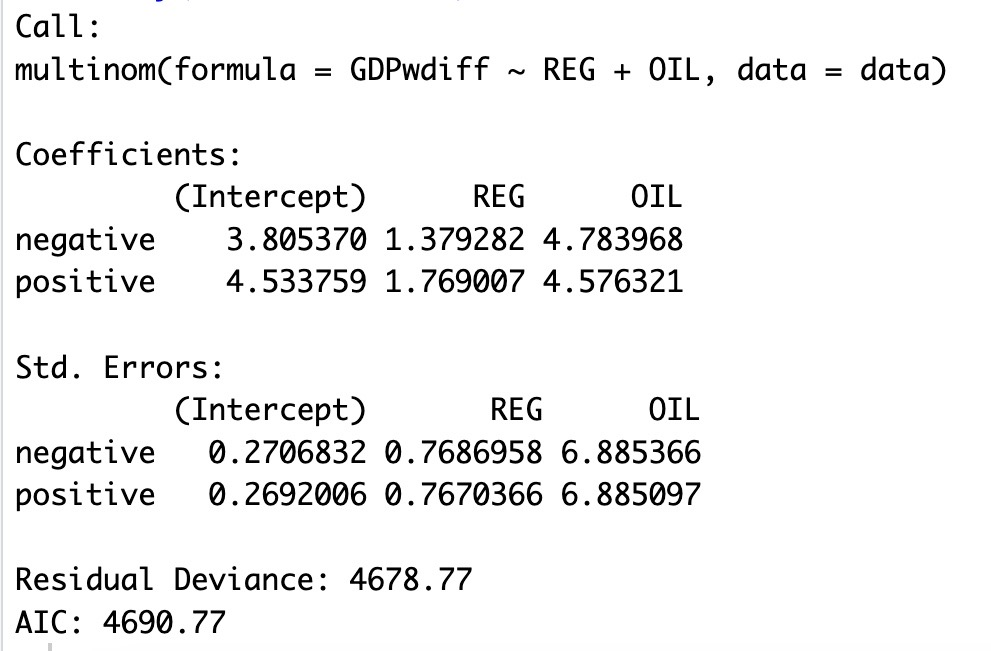
\includegraphics[width=0.8\textwidth]{unordered_1.jpg}
\linebreak
\lstinputlisting[language=R, firstline=29, lastline=35]{PS3.R} 
\textbf{Cut-off-points:}
\linebreak
	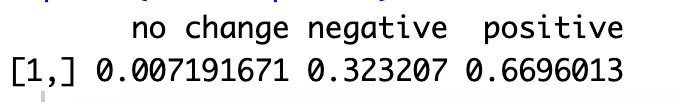
\includegraphics[width=0.6\textwidth]{unordered_2.jpg}
\linebreak
\textbf{Interpretation:}
\linebreak
In an unordered multinomial model, the coefficients represent the change in the log-odds of moving from one category to a specific reference category. The unordered multinomial logistic regression model aims to predict the outcome variable 'GDPwdiff', which has three (unordered) categories -  ‘no change’, ‘negative’, and ‘positive’. The coefficients in the summary output represent the estimated log odds of being in each category, relative to the reference category - which in this case is the ’no change’ category. 

For the ‘negative’ category, the intercept is 3.805370, meaning that the log odds of being in the negative category, relative to the reference category (‘no change’), are 3.805370 when both REG and OIL are equal to 0. Further, for one-unit increase in REG, the log odds of being in the negative category increase by 1.379282, and for one-unit increase in OIL, the log odds of being in the negative category increase by 4.783968.

The same interpretation applies to the positive category and its coefficients.

The cutoff points represent the thresholds for the predicted probabilities that determine which outcome category is most likely given the predictor values. For example, for the first predictor variable, if the predicted probability of "no change" is less than 0.007, the model predicts that the outcome will be "negative". If the predicted probability of "no change" is greater than 0.669, the model predicts that the outcome will be "positive". If the predicted probability of "no change" falls between these two cutoff points, the model predicts that the outcome will be "no change".
These cutoff points are useful for interpreting the model's predictions based on the model's outputs.

	\item Construct and interpret an ordered multinomial logit with \texttt{GDPWdiff} as the outcome variable, including the estimated cutoff points and coefficients.
\linebreak
\lstinputlisting[language=R, firstline=38, lastline=45]{PS3.R} 
\textbf{Coefficients: }
\linebreak
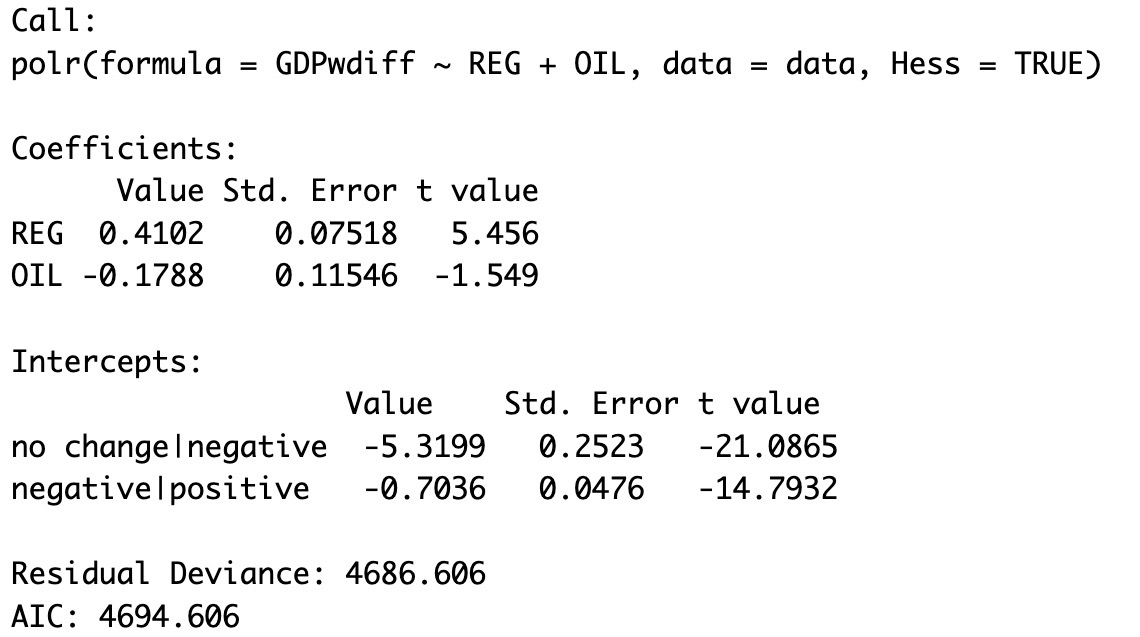
\includegraphics[width=0.8\textwidth]{ordered_1.jpg}
\linebreak
\lstinputlisting[language=R, firstline=47, lastline=53]{PS3.R} 
\textbf{Cut-off-points:}
\linebreak
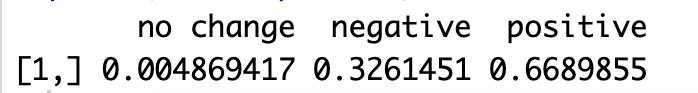
\includegraphics[width=0.6\textwidth]{ordered_2.jpg}
\linebreak

\textbf{Interpretation:}
\linebreak
In an ordered multinomial model, the coefficients represent the change in the log-odds of moving from one category to the next higher category. For example, the coefficient for REG in the 'no change' category represents the change in the log-odds of moving from 'no change' to 'negative' category. 

This model is trying to predict whether GDPwdiff will be 'no change', 'negative', or 'positive' based on two variables called REG and OIL. The coefficient for REG is 0.4102, which means that for each one-unit increase in REG, the likelihood of GDPwdiff being in the 'no change' category increases by 0.4102. The coefficient for OIL is -0.1788, which means that for each one-unit increase in OIL, the likelihood of GDPwdiff being in the 'no change' category decreases by 0.1788.

The intercepts represent the starting point for each category of GDPwdiff. The intercept for the 'no change' category is -5.3199, which means that if REG and OIL are both 0, the likelihood of GDPwdiff being in the 'no change' category is very high. The intercept for the 'negative' category is -0.7036, which means that if REG and OIL are both 0, the likelihood of GDPwdiff being in the 'negative' category is relatively high.

In an ordered multinomial logistic regression model, the cutoff points are the thresholds for the predicted probabilities that determine which outcome category is most likely given the predicted cut-off points. For example, if the predicted probability of 'no change' is less than 0.004869417, the model predicts that the outcome will be 'negative'. If the predicted probability of 'no change' is greater than 0.6689855, the model predicts that the outcome will be 'positive'. If the predicted probability of 'no change' falls between these two cutoff points, the model predicts that the outcome will be 'no change'.
	
\end{enumerate}

\section*{Question 2} 
\vspace{.25cm}

\noindent Consider the data set \texttt{MexicoMuniData.csv}, which includes municipal-level information from Mexico. The outcome of interest is the number of times the winning PAN presidential candidate in 2006 (\texttt{PAN.visits.06}) visited a district leading up to the 2009 federal elections, which is a count. Our main predictor of interest is whether the district was highly contested, or whether it was not (the PAN or their opponents have electoral security) in the previous federal elections during 2000 (\texttt{competitive.district}), which is binary (1=close/swing district, 0="safe seat"). We also include \texttt{marginality.06} (a measure of poverty) and \texttt{PAN.governor.06} (a dummy for whether the state has a PAN-affiliated governor) as additional control variables. 

\begin{enumerate}
	\item [(a)]
	Run a Poisson regression because the outcome is a count variable. Is there evidence that PAN presidential candidates visit swing districts more? Provide a test statistic and p-value.
\lstinputlisting[language=R, firstline=63, lastline=70]{PS3.R} 
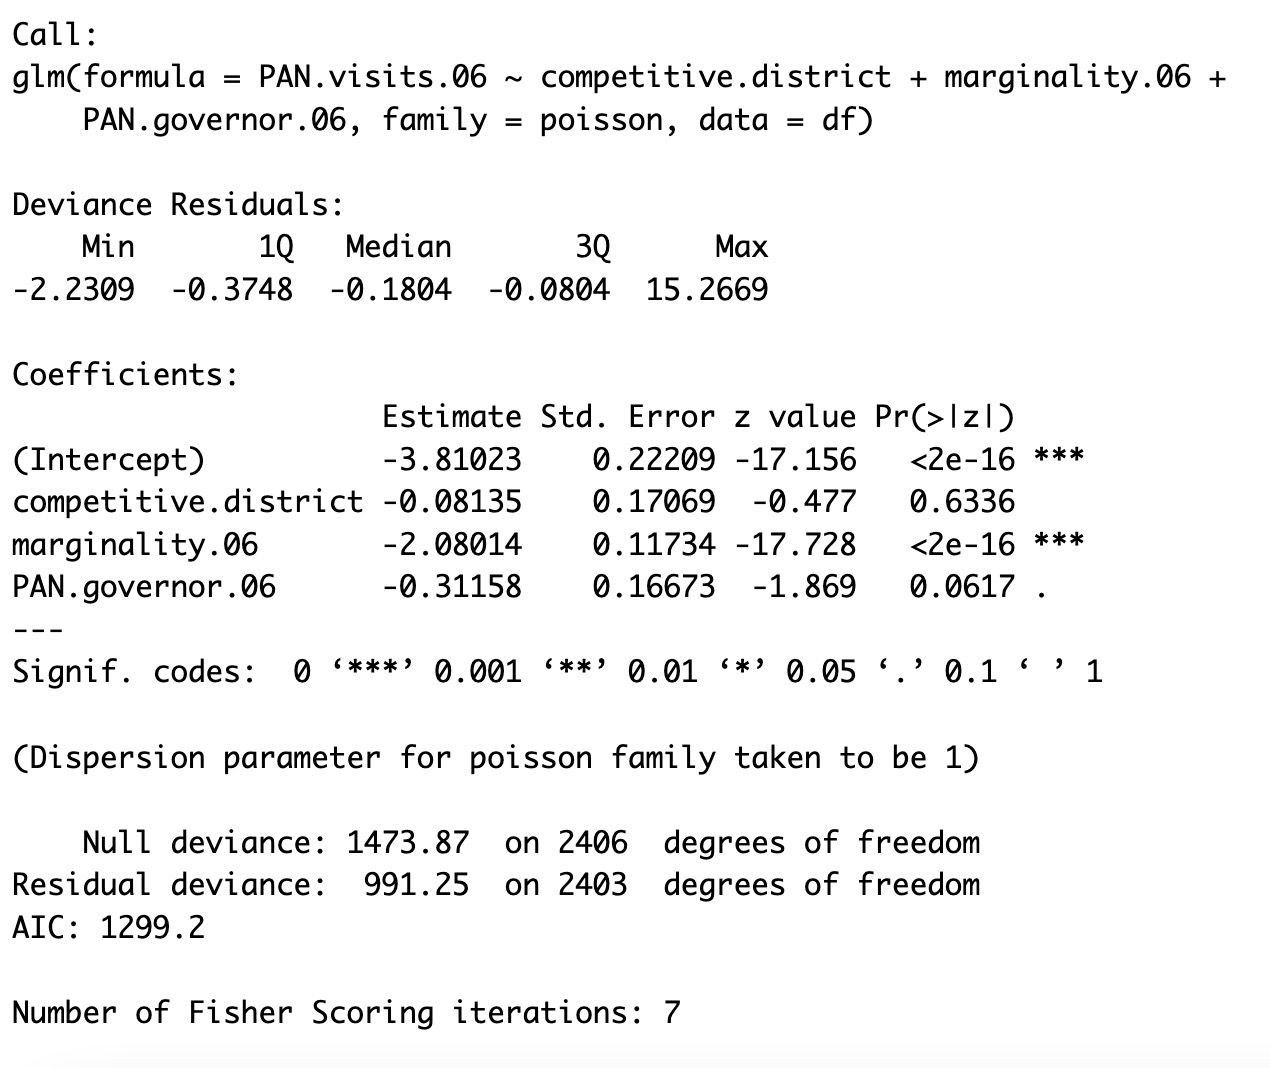
\includegraphics[width=1\textwidth]{Poisson_regression.jpg}

Based on the output of the Poisson regression, we can see that the coefficient estimate for competitive.district is negative (-0.08135) and not statistically significant (p-value = 0.6336), which suggests that there is no evidence to support the claim that PAN presidential candidates visit swing districts more. The test statistic for the Poisson model is the z-value. The z-value is given for each coefficient in the "Coefficients" table under the column "z value". 
	\item [(b)]
	Interpret the \texttt{marginality.06} and \texttt{PAN.governor.06} coefficients.
	
	The coefficient for marginality.06 in the Poisson regression model is -2.08014. This indicates that for a one-unit increase in marginality, holding all other variables constant, the expected log count of PAN presidential candidate visits decreases by 2.08014. 
	
	The coefficient for PAN.governor.06 is -0.31158. This means that for a one-unit increase in the presence of a PAN governor in a district, holding all other variables constant, the expected log count of PAN presidential candidate visits decreases by 0.31158.
	
	\item [(c)]
	Provide the estimated mean number of visits from the winning PAN presidential candidate for a hypothetical district that was competitive (\texttt{competitive.district}=1), had an average poverty level (\texttt{marginality.06} = 0), and a PAN governor (\texttt{PAN.governor.06}=1).
	\lstinputlisting[language=R, firstline=84, lastline=85]{PS3.R} 
	
	[1] 0.01494827
	
	This means that on average, the winning PAN presidential candidate is estimated to make 0.0149 visits to a hypothetical district with the given characteristics.
	
	
	
\end{enumerate}

\end{document}
